\doublespacing
\chapter{Conclusions}\label{chap:conclusions}
%\version{v1.10.2015}
The conclusion of our final year project is describe below.
\section{Project Conclusion}
Food conservation and waste reduction is a web application in which a company or organization having products near to the expire date or any hotels or marquees having excess food can simply register in our web application and then they upload details about the product, set the price of bid and place end time for the bid. The seller will be shown top bids and the one with the highest bid will win the product and user will be sent to payment page for further processing and finally user can pick the product from given location.
\section{Limitations}
\textbf{1} : Internet connection is always required to access the data from our website.\\
\textbf{2} : The slow speed of loading of online picture contents when retrieved from data base.\\
\textbf{3} : Security risk posed by threat vectors.

\section{User Guide}
The user guide contains step by step process of using our web application form registration in web application to buy the product in the system.\\
\subsection{Home Page}
When user visit in our web application he will enter to home page. The home page of our web application is shown in following Figure \ref{HPl}.All the information about bidding will be shown in home page. He can place bid only if he is login in our web application. In case of invalid URL in search. The Visitors  will be moved to 404 not found page which angular provide as wild card in routing and navigation listed at the last of routing.\\
\begin{figure}[h]
    \centering
    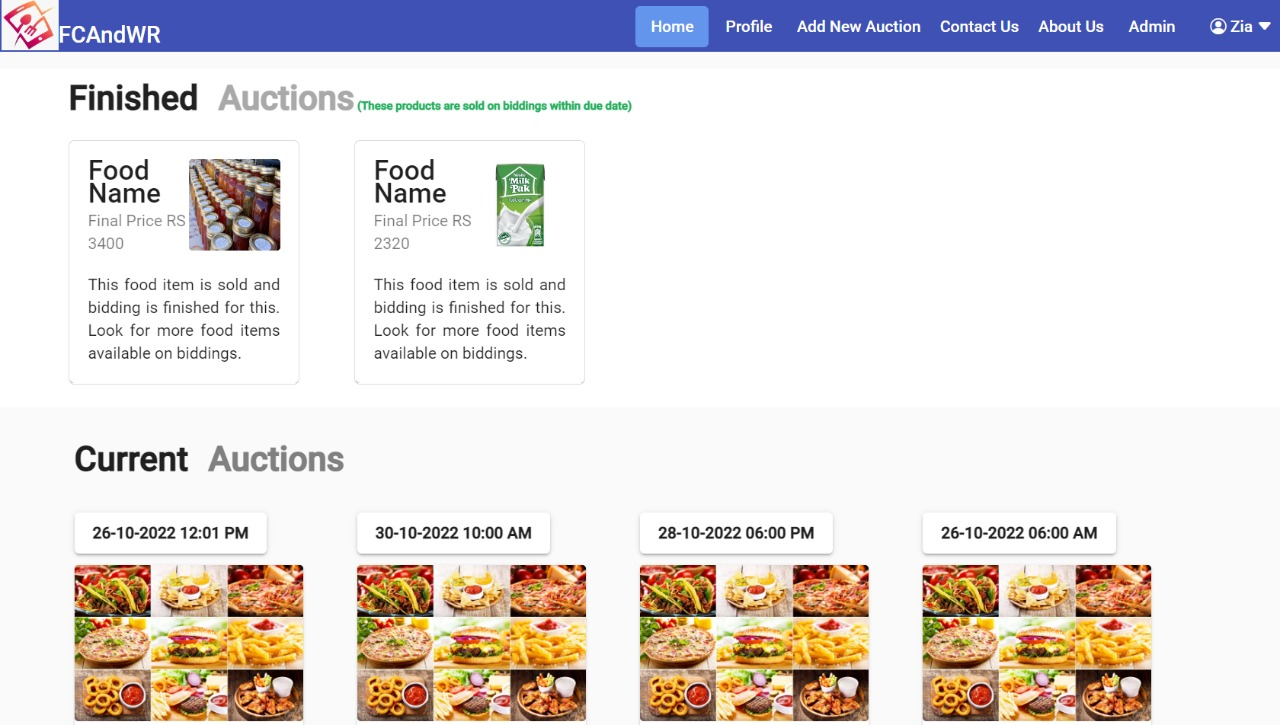
\includegraphics[width=15cm, height=15cm, keepaspectratio]{Homepage.jpeg}
    \caption{Home Page}
    \label{HPl}
\end{figure}
\subsection{Login Page}
After successfully getting register into our web application, user simply need to enter his email and password for login. The login page of our web application is shown in following Figure \ref{lp}.\\
\begin{figure}[!h]
    \centering
    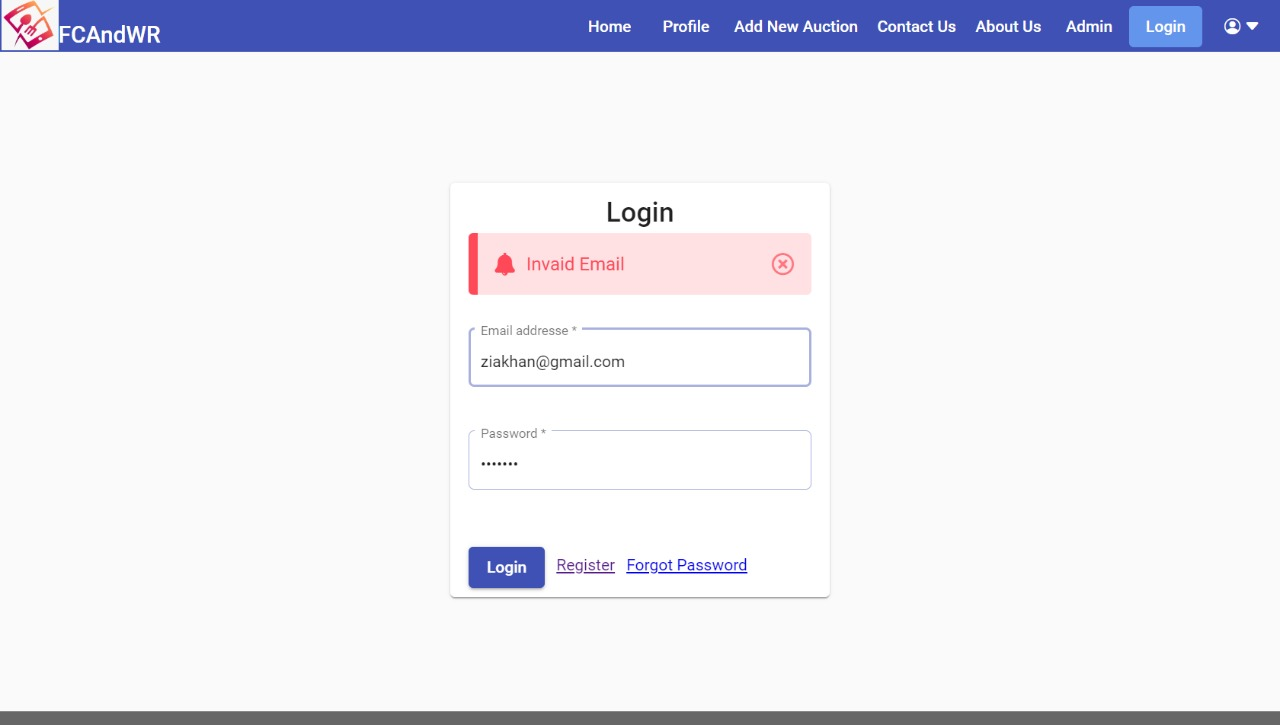
\includegraphics[width=15cm, height=15cm, keepaspectratio]{login page.jpeg}
    \caption{Login Page}
    \label{lp}
\end{figure}
\newpage
\subsection{Login Page Requirements}
If user will Press the login button, then an error will be thrown to him to notify that he must fill all the required credentials. The login page with required field of our web application is shown in following Figure \ref{Lrf}.
\begin{figure}[!h]
    \centering
    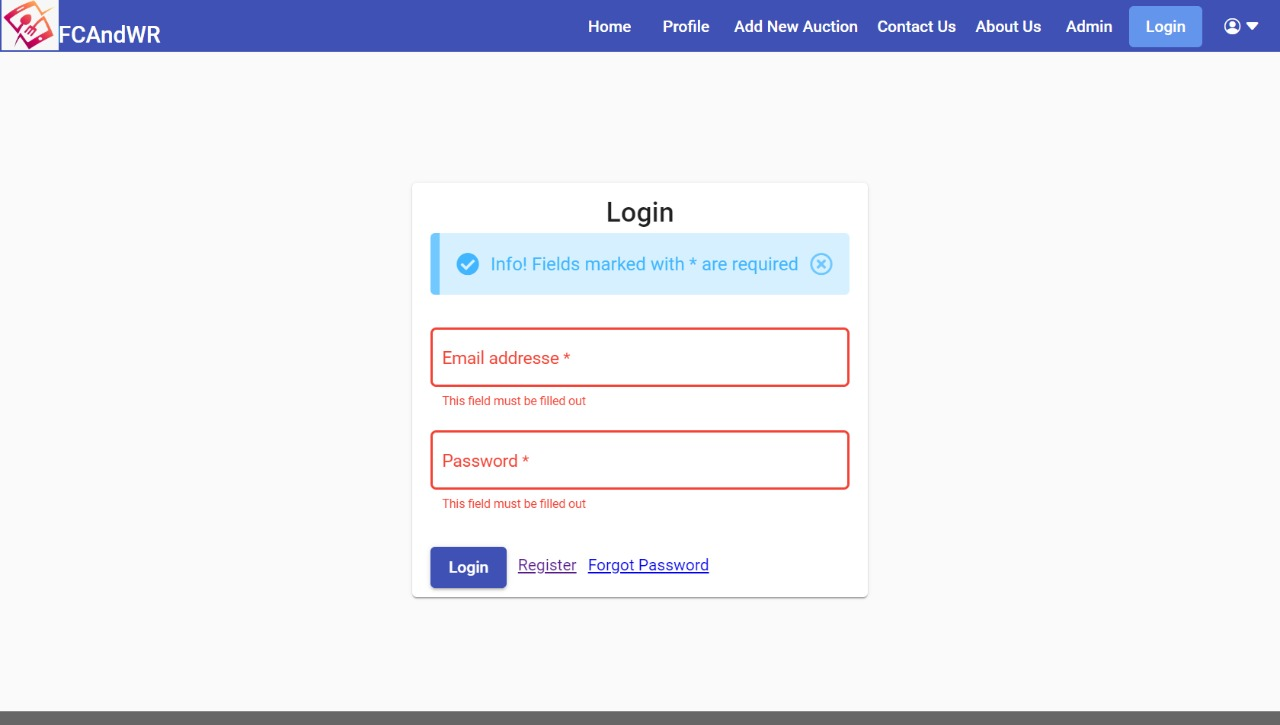
\includegraphics[width=15cm, height=15cm, keepaspectratio]{Login required.jpeg}
    \caption{Responsive Login Page}
    \label{Lrf}
\end{figure}


\subsection{Registration Page}
If the user wants to perform bidding or take part in it, he will first register in application by entering his name, phone number, email address, city, and his address. The registration page of our web application is shown in following Figure \ref{rp}.\\
\begin{figure}[!h]
    \centering
    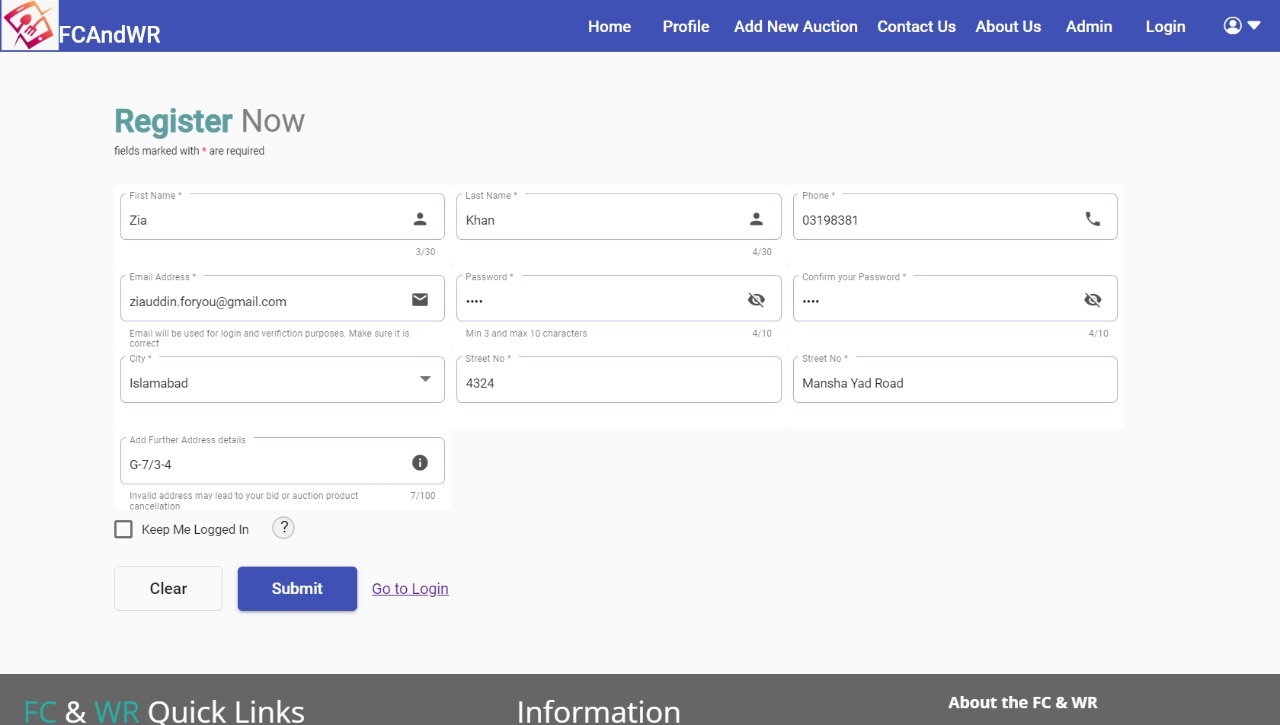
\includegraphics[width=15cm, height=15cm, keepaspectratio]{Register Page.jpeg}
    \caption{Register Page}
    \label{rp}
\end{figure}

\subsection{Registration Page Requirements}
If user will press the login button, then an error will be thrown to him to notify that he must fill all the required credentials. The registration page with requirements of our web application is shown in following Figure \ref{rpr}.
\begin{figure}[!h]
    \centering
    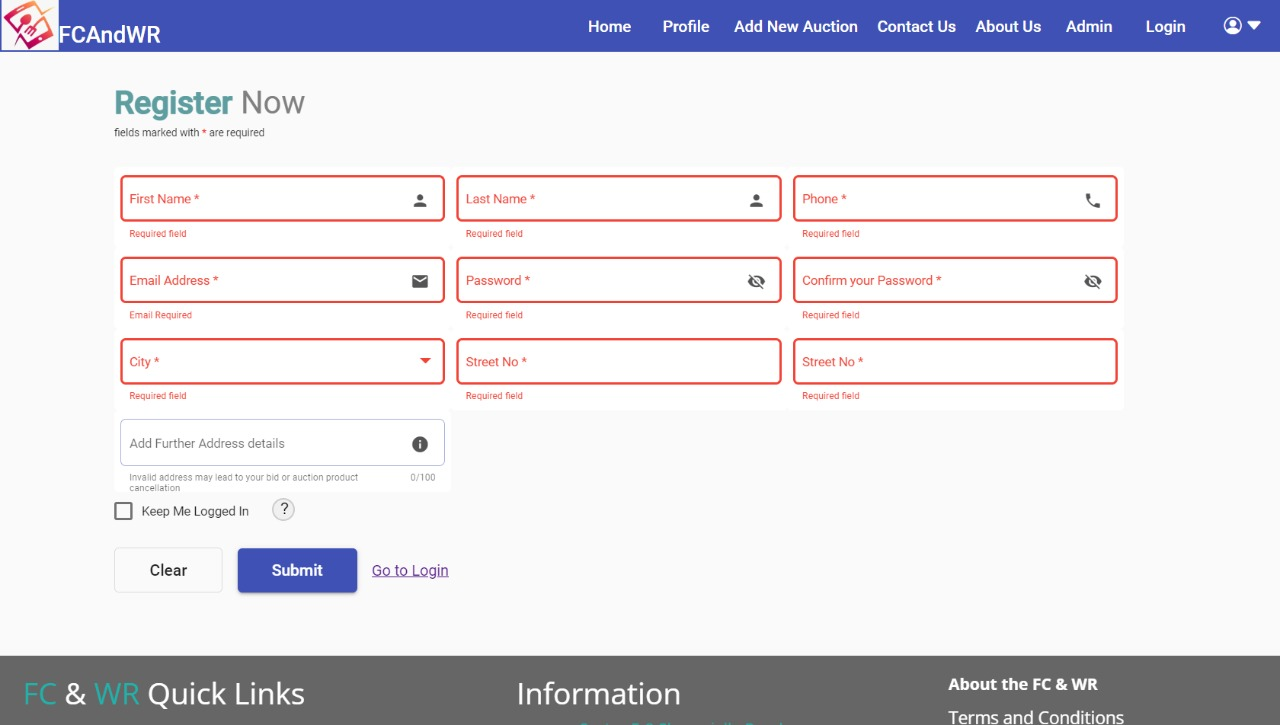
\includegraphics[width=15cm, height=15cm, keepaspectratio]{Responsive register page.jpeg}
    \caption{Responsive Registration}
    \label{rpr}
\end{figure}
\newpage
\subsection{Forgot Password}
If user forgets his password, then he will be sent a code to his registered email where he can recover his password. The forgot password page of our web application is shown in following Figure \ref{fp}.\\\\
\begin{figure}[!h]
    \centering
    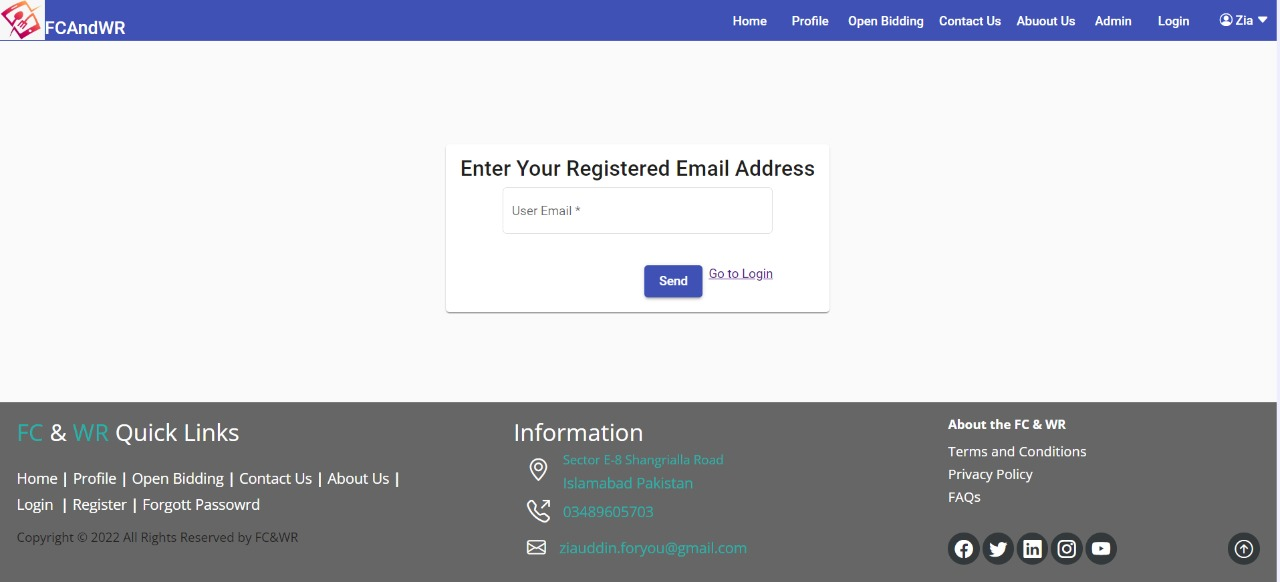
\includegraphics[width=15cm, height=15cm, keepaspectratio]{projectReportTemplate/figures/forgot.jpeg}
    \caption{Reset Password}
    \label{fp}
\end{figure}


\subsection{Profile Page}
This page shows the user purchase history and user sales history. when a user won a bid he will be able to see his won bid in his profile section. The profile page of our web application is shown in following Figure \ref{pp}.
\begin{figure}[!h]
    \centering
    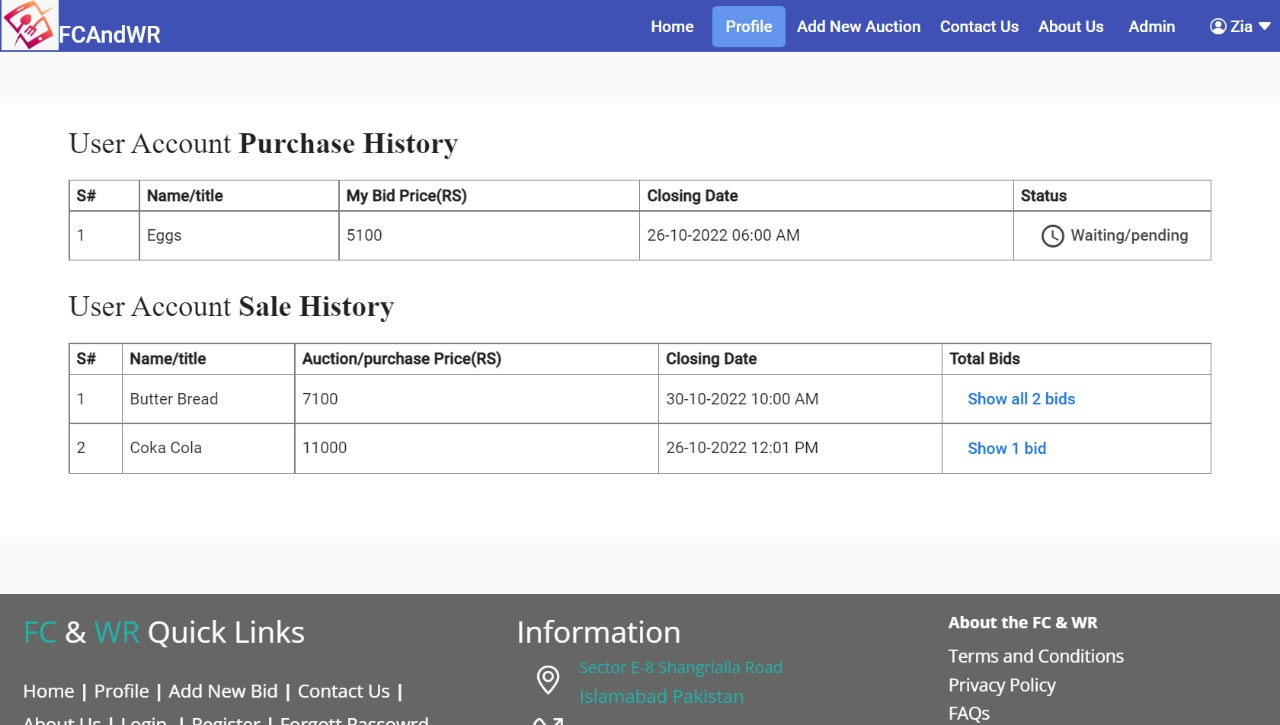
\includegraphics[width=15cm, height=15cm, keepaspectratio]{profile.jpeg}
    \caption{Profile Page}
    \label{pp}
\end{figure}

\subsection{Non-Login Profile Page}
This page shows the user purchase history and user sales history. when a user won a bid he will be able to see his won bid in his profile section. The non-login profile page of our web application is shown in following Figure \ref{nlpp}.
\begin{figure}[!h]
    \centering
    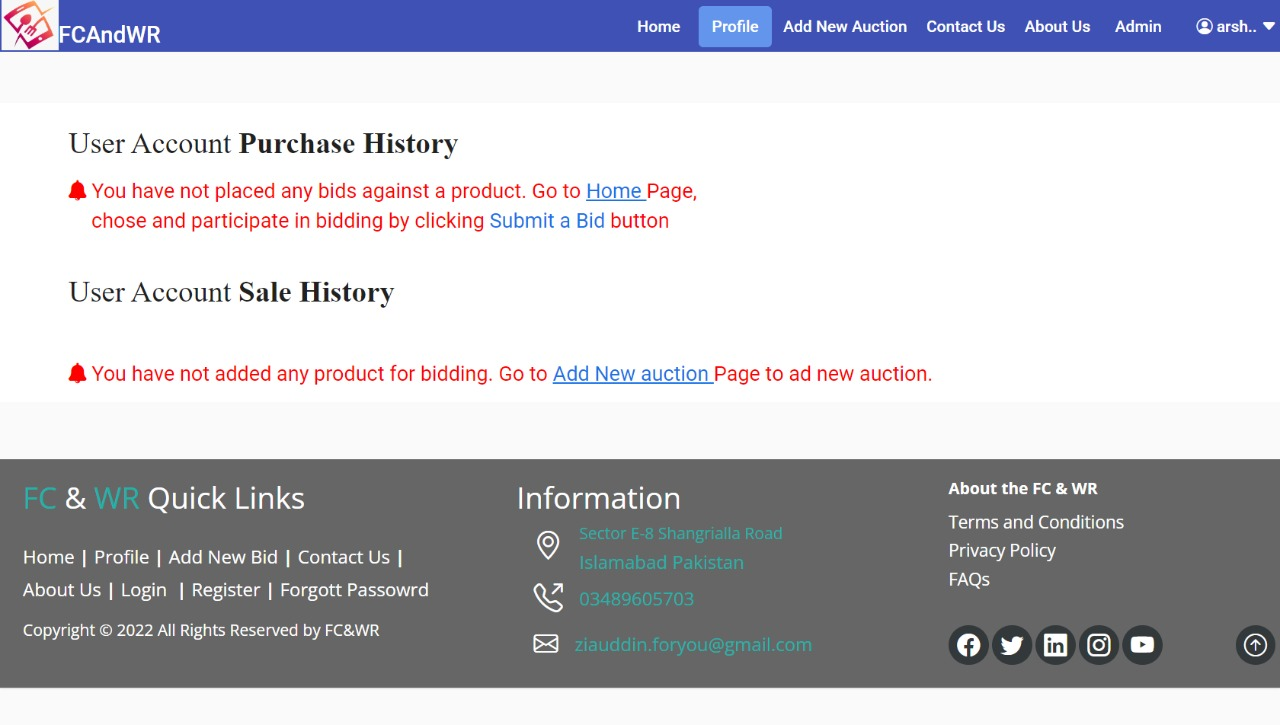
\includegraphics[width=15cm, height=15cm, keepaspectratio]{unlogin profile page.jpeg}
    \caption{Non-Login Profile Page}
    \label{nlpp}
\end{figure}
\newpage

\subsection{Checkout/Payment Page}
This page show the user purchase history and user sales history. when a user won a bid. He will be able to see his won bid in his profile section. The payment page of our web application is shown in following Figure \ref{co}.\\
\begin{figure}[!h]
    \centering
    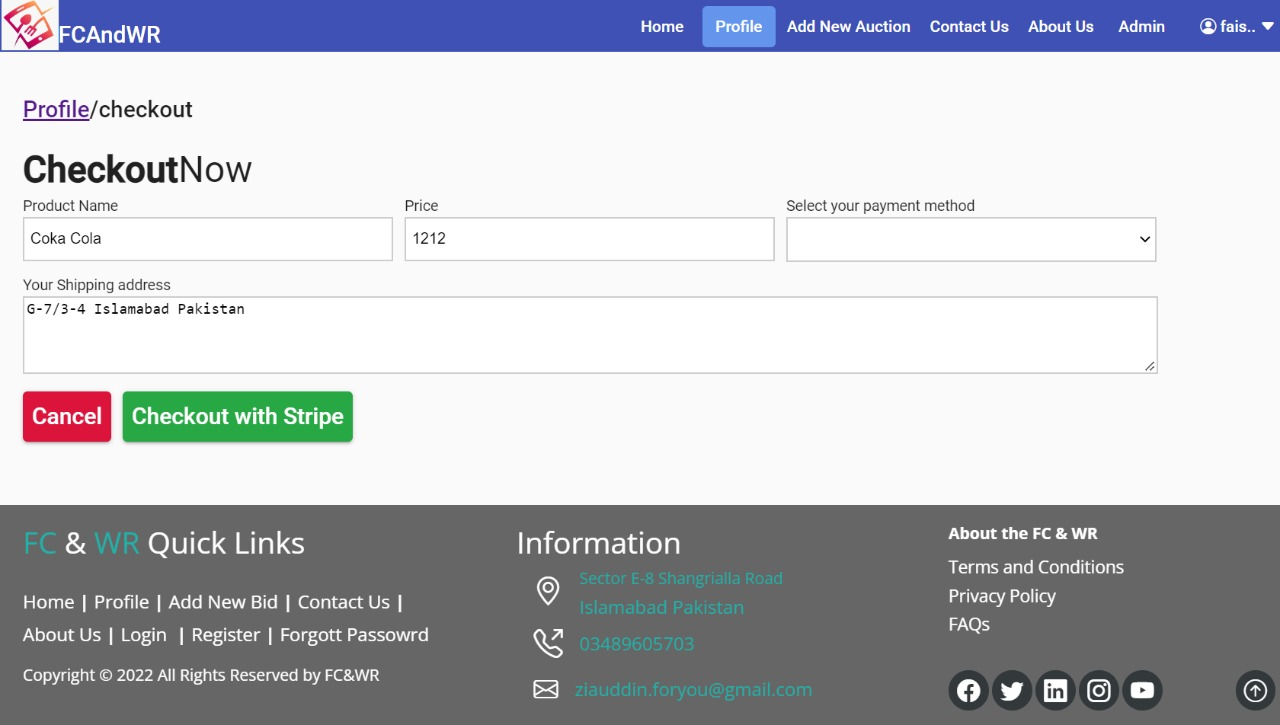
\includegraphics[width=15cm, height=15cm, keepaspectratio]{Checkout page.jpeg}
    \caption{Checkout/Payment Page}
    \label{co}
\end{figure}
\newpage
\subsection{Add New Auction Page}
In this page user will be able to add the information regarding the product he want to place on the bidding. He will enter product name, set it's price for auction and his address details. Finally he will add picture of the product and submit for new bid. The add new auction page of our web application is shown in following Figure \ref{ano}.\\\\
\begin{figure}[!h]
    \centering
    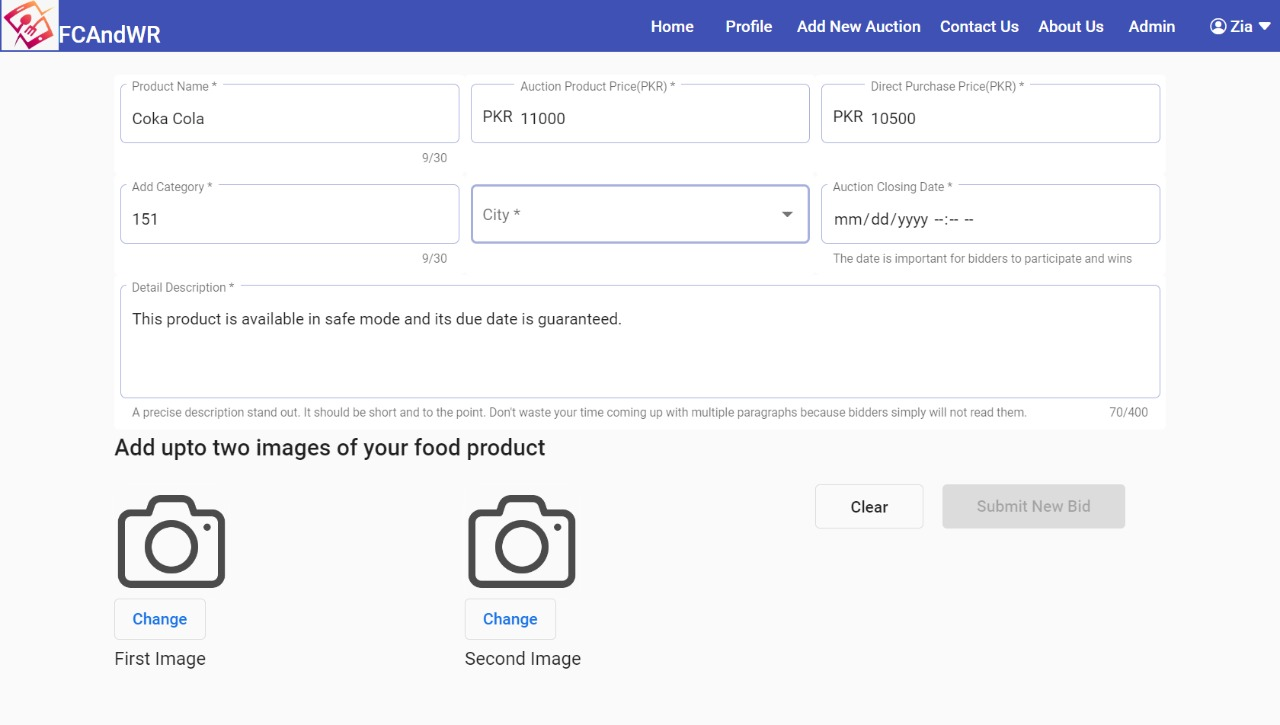
\includegraphics[width=15cm, height=15cm, keepaspectratio]{add new auction.jpeg}
    \caption{Add New Auction Page}
    \label{ano}
\end{figure}
\newpage
\subsection{Bid Detail Page}
In this page the buyer will be able to see the details of the product on auction and also he will be able to see time left for the bid. If he is interested then he will be able to place the bid. The bid detail page of our web application is shown in following Figure \ref{bdp}.\\\\
\begin{figure}[!h]
    \centering
    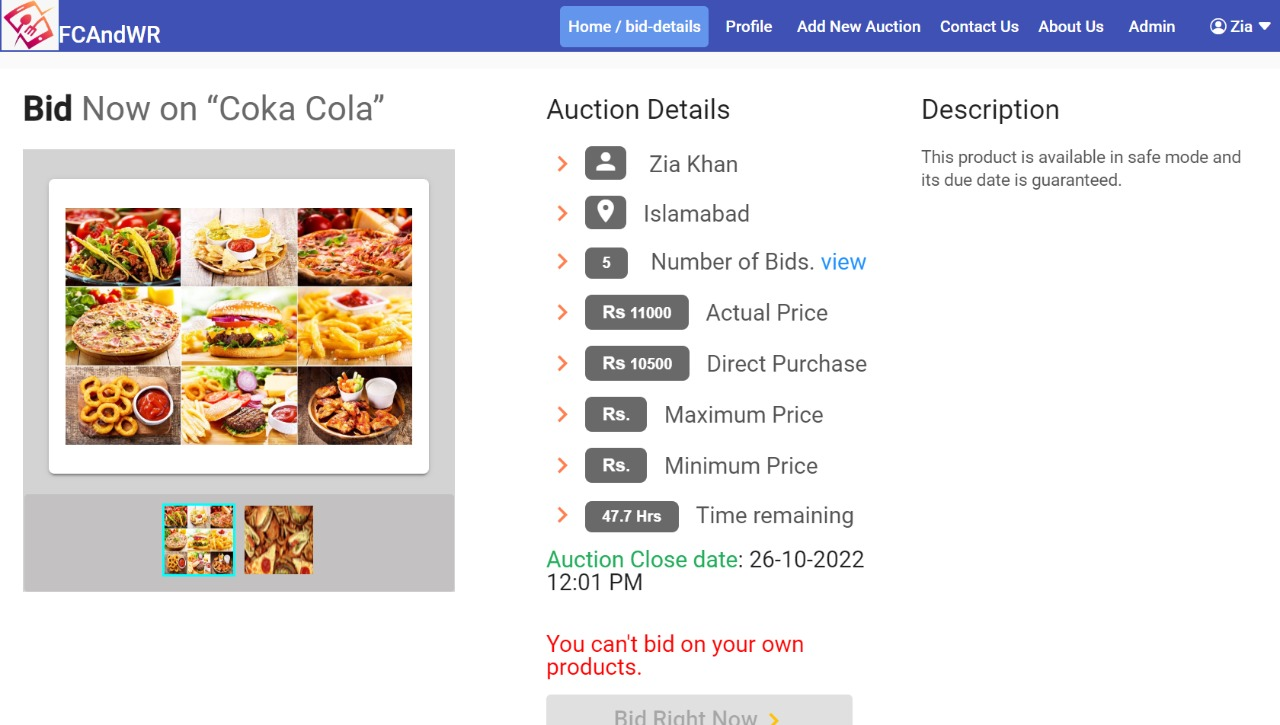
\includegraphics[width=15cm, height=15cm, keepaspectratio]{Bid details.jpeg}
    \caption{Bid Detail Page}
    \label{bdp}
\end{figure}
\newpage
\subsection{Bid Detail Update Page}
This is the extension of bid page when buyer select submit the bid then he enters the bid price that how much he is willing to pay for the product and also he can add a comment. The bid detail update page of our web application is shown in following Figure \ref{dbuo}.\\\\
\begin{figure}[!h]
    \centering
    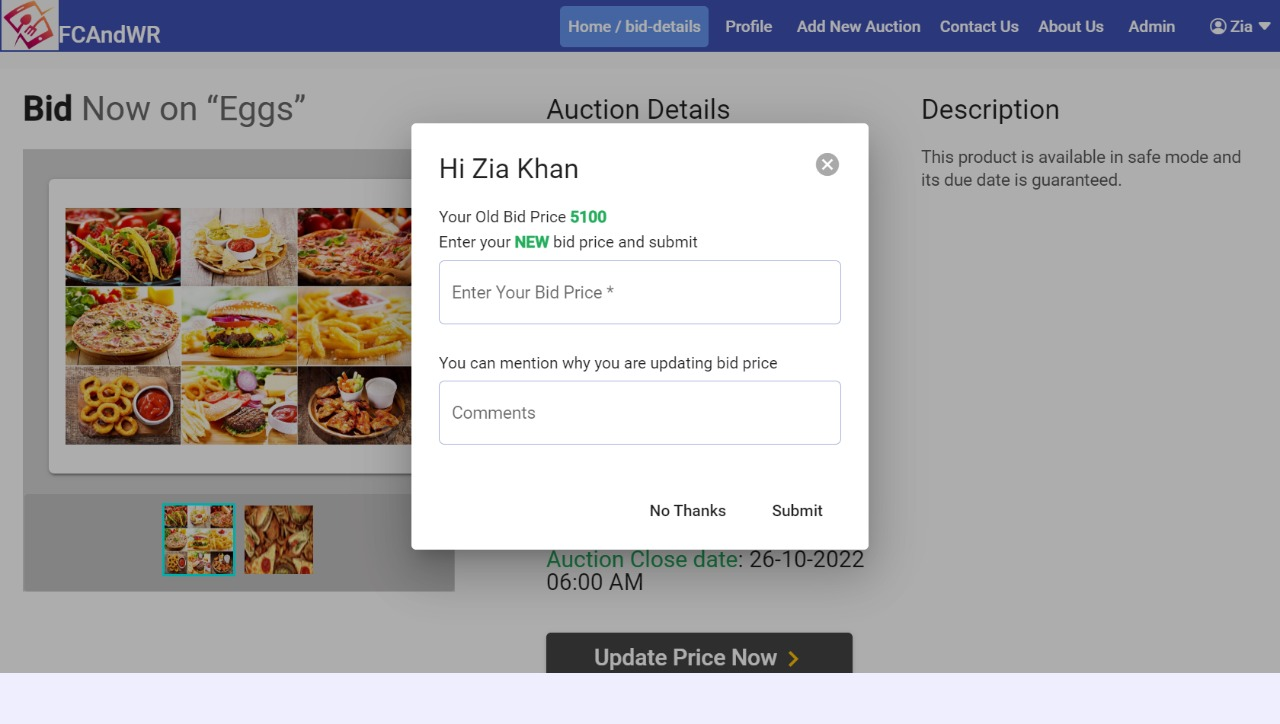
\includegraphics[width=15cm, height=15cm, keepaspectratio]{Bid details update.jpeg}
    \caption{Bid Detail Update Page}
    \label{dbuo}
\end{figure}
\newpage
\subsection{Contact Us Page}
If the user have an quarry then he can contact is through this page. The contact us page of our web application is shown in following Figure \ref{cu}.
\begin{figure}[!h]
    \centering
    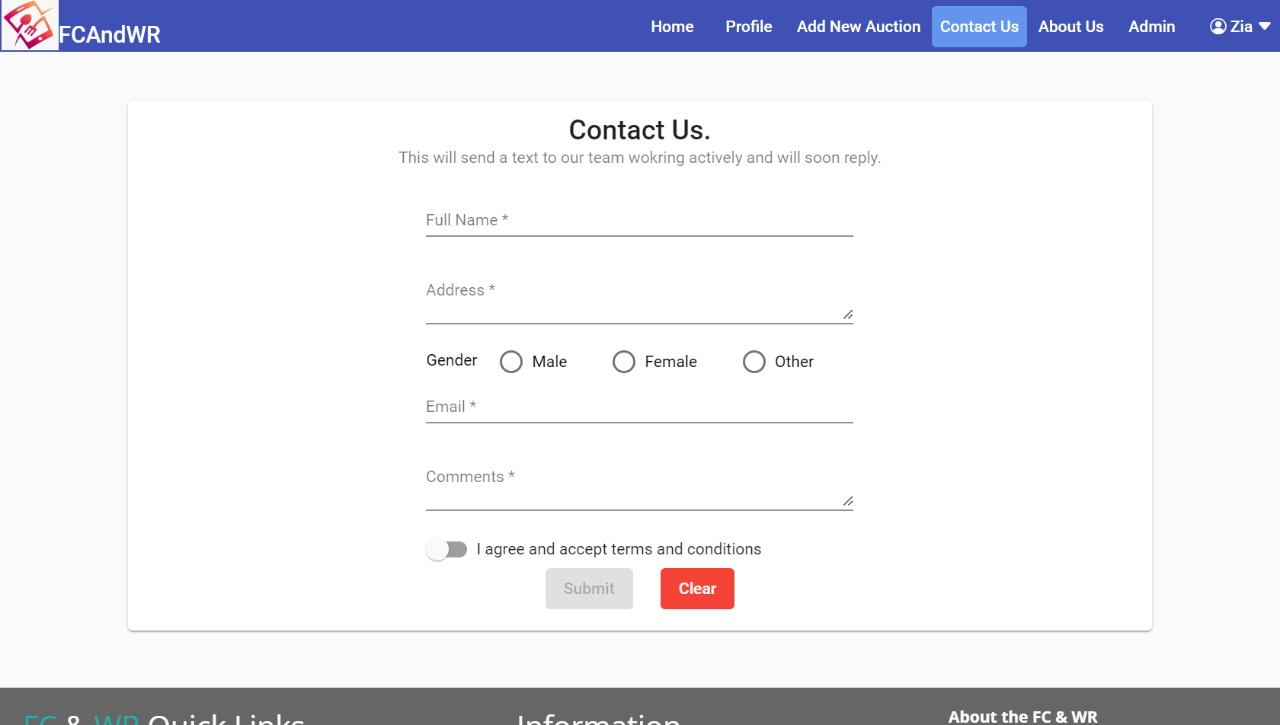
\includegraphics[width=15cm, height=15cm, keepaspectratio]{Contact us.jpeg}
    \caption{Contact Us Page}
    \label{cu}
\end{figure}